\chapter{\RU{Ф-ция toupper()}\EN{toupper() function}}
\index{\CStandardLibrary!toupper()}

\RU{Еще одна очень востребованная функция конвертирует символ из строчного в заглавный, если нужно:}
\EN{Another very popular function transforms symbol from lower case to upper case, if needed:}

\lstinputlisting{\CURPATH/toupper.c}

\RU{Выражение \TT{'a'+'A'} оставлено в исходном коде для удобства чтения, 
конечно, оно соптимизируется}
\EN{\TT{'a'+'A'} expression is left in source code for better readability, it is to be 
optimized by compiler, of course}
\footnote{
\RU{Впрочем, если быть дотошным, я думаю, вполне могут до сих пор существовать компиляторы,
которые не оптимизируют подобное и оставляют в коде.}
\EN{However, if to be meticulous, I think, there are still could be compilers which can't optimize such expressions
and leaving them right in the code.}}.

\EN{The \ac{ASCII} code of \q{a} symbol is 97 (or 0x61), and 65 (or 0x41) for \q{A} symbol.}
\RU{\ac{ASCII}-код символа \q{a} это 97 (или 0x61), и 65 (или 0x41) для символа \q{A}.}
\EN{The difference (or distance) between them in \ac{ASCII} table is 32 (or 0x20).}
\RU{Разница (или расстояние) между ними в \ac{ASCII}-таблица это 32 (или 0x20).}

\EN{For better understanding, reader may take a look at 7-bit standard \ac{ASCII} table:}
\RU{Для лучшего понимания, читатель может посмотреть на стандартную 7-битную таблицу \ac{ASCII}:}

\begin{figure}[H]
\centering
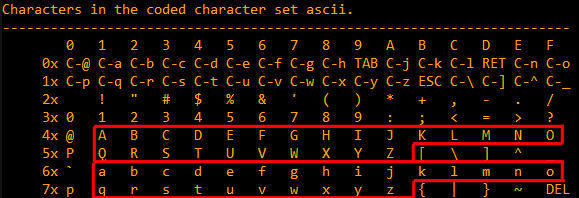
\includegraphics[scale=\FigScale]{\CURPATH/ascii.png}
\caption{\EN{7-bit \ac{ASCII} table in Emacs}\RU{7-битная таблица \ac{ASCII} в Emacs}}
\end{figure}

\section{x64}

\subsection{\EN{Two comparison operations}\RU{Две операции сравнения}}

\EN{\NonOptimizing MSVC is straightforward: the code checks if input symbol is in [97..122] range 
(or in [`a'..`z'] range) and subtracts 32 in this case.}
\RU{\NonOptimizing MSVC прямолинеен: код проверят, находится ли входной символ в интервале [97..122]
(или в интервале [`a'..`z'] ) и вычитает 32 в таком случае.}
\EN{There are also minor compiler artefact:}
\RU{Имеется также небольшой артефакт компилятора:}

\lstinputlisting[caption=\NonOptimizing MSVC 2013 (x64),numbers=left]{\CURPATH/MSVC_2013_x64.asm}

\EN{It's important to notice that input byte is loaded into 64-bit local stack slot at line 3.}
\RU{Важно отметить что (на строке 3) входной байт загружается в 64-битный слот локального стека.}
\EN{All the rest bits ([8..63]) are untouched, i.e., contains some random noise (you'll see it in debugger).}
\RU{Все остальные биты ([8..63]) не трогаются, т.е. содержат случайный шум (вы можете увидеть его в отладчике).}
% TODO add debugger example
\EN{All instructions operates only on byte-level, so it's fine.}
\RU{Все инструкции работают только с байтами, так что всё нормально.}
\EN{The last \TT{MOVZX} instruction at line 15 takes byte from local stack slot and zero-extends it into \Tint 
32-bit data type.}
\RU{Последняя инструкция \TT{MOVZX} на строке 15 берет байт из локального стека и расширяет его 
до 32-битного \Tint, дополняя нулями.}

\NonOptimizing GCC \EN{does mostly the same}\RU{делает почти то же самое}:

\lstinputlisting[caption=\NonOptimizing GCC 4.9 (x64)]{\CURPATH/GCC_49_x64_O0.s}

\subsection{\EN{One comparison operation}\RU{Одна операция сравнения}}
\label{toupper_one_comparison}

\Optimizing MSVC \EN{does its job better, it generates only one comparison operation}\RU{работает лучше,
он генерирует только одну операцию сравнения}:

\lstinputlisting[caption=\Optimizing MSVC 2013 (x64)]{\CURPATH/MSVC_2013_Ox_x64.asm}

\EN{It was explained earlier, how to replace two comparison operations by one}
\RU{Я уже описывал, как можно заменить две операции сравнения на одну}: \myref{one_comparison_instead_of_two}.

\EN{I would rewrite this into \CCpp:}
\RU{Я бы переписал это на \CCpp так:}

\begin{lstlisting}
int tmp=c-97;

if (tmp>25)
        return c;
else
        return c-32;
\end{lstlisting}

\EN{\IT{tmp} variable should be signed.}
\RU{Переменная \IT{tmp} должна быть знаковая.}
\EN{This makes two subtracting operations in case of transformation plus one comparison operation.}
\RU{При помощи этого, имеем две операции вычитания в случае конверсии плюс одну операцию сравнения.}
\EN{While original algorithm uses two comparison operations plus one subtracting operation.}
\RU{В то время как оригинальный алгоритм использует две операции сравнения плюс одну операцию вычитания.}

\Optimizing GCC \EN{is even better, it got rid of jumps (which is good: \myref{branch_predictors}) 
by using CMOVcc instruction:}
\RU{даже лучше, он избавился от переходов (а это хорошо: \myref{branch_predictors}) используя инструцкию CMOVcc:}

\lstinputlisting[caption=\Optimizing GCC 4.9 (x64),numbers=left]{\CURPATH/GCC_49_x64_O3.s}

\EN{At line 3 the code prepares the subtracted value in advance, as if conversion will happen always.}
\RU{На строке 3 код готовит уже сконвертированное значение заранее, как если бы коверсия всегда происходила.}
\EN{At line 5 subtracted value in EAX is replaced by untouched input value if conversion is not needed.
And then this value (of course incorrect) is dropped.}
\RU{На строке 5 это значение в EAX заменяется нетронутым входным значением, если конверсия не нужна.
И тогда это значение (конечно, неверное), просто выбрасывается.}
\EN{Advance subtracting is a price compiler paying for the absence of conditional jumps.}
\RU{Вычитание с упреждением это цена, которую компилятор платит за отсутствие условных переходов.}

\section{ARM}

\EN{\Optimizing Keil for ARM mode also generates only one comparison:}
\RU{\Optimizing Keil для режима ARM также генерирует только одну операцию сравнения:}

\lstinputlisting[caption=\OptimizingKeilVI (\ARMMode)]{\CURPATH/Keil_ARM_O3.s}

\index{ARM!\Instructions!SUBcc}
\index{ARM!\Instructions!ANDcc}
\EN{SUBLS and ANDLS instructions are executing only if \Reg{1} value is less than 0x19 (or equal).
They do actual conversion.}
\RU{SUBLS и ANDLS исполняются только если значение \Reg{1} меньше чем 0x19 (или равно).
Они и делают конверсию.}

\EN{\Optimizing Keil for Thumb mode generates only one comparison operation as well:}
\RU{\Optimizing Keil для режима Thumb также генерирует только одну операцию сравнения:}

\lstinputlisting[caption=\OptimizingKeilVI (\ThumbMode)]{\CURPATH/Keil_thumb_O3.s}

\index{ARM!\Instructions!LSLS}
\index{ARM!\Instructions!LSLR}
\EN{Last two LSLS and LSRS instructions works like \TT{AND reg, 0xFF}:
they are analogous to \CCpp-expression $(i<<24)>>24$.}
\RU{Последние две инструкции LSLS и LSRS работают как \TT{AND reg, 0xFF}:
это аналог \CCpp-выражения $(i<<24)>>24$.}
\EN{Apparently, Keil for Thumb mode deduced that two 2-byte instructions is shorter then the code 
loading 0xFF constant into register plus AND instruction.}
\RU{Очевидно, Keil для режима Thumb решил что две 2-байтных инструкции это короче чем код, загружающий
константу 0xFF плюс инструкция AND.}

\subsection{GCC \ForENRU ARM64}

\lstinputlisting[caption=\NonOptimizing GCC 4.9 (ARM64)]{\CURPATH/GCC_49_ARM64_O0.s}

\lstinputlisting[caption=\Optimizing GCC 4.9 (ARM64)]{\CURPATH/GCC_49_ARM64_O3.s}

\section{\EN{Summary}\RU{Итог}}

\EN{All these compiler optimizations are very popular nowadays 
and practicing reverse engineer usually sees such code patterns often.}
\RU{Все эти оптимизации компиляторов очень популярны в наше время и практикующий
reverse engineer обычно часто видит такие варианты кода.}
